%% LyX 2.3.7 created this file.  For more info, see http://www.lyx.org/.
%% Do not edit unless you really know what you are doing.
\documentclass[journal,article,submit,pdftex,moreauthors]{Definitions/mdpi}
\usepackage[utf8]{inputenc}
\usepackage{float}
\usepackage{url}
\usepackage{amsmath}
\usepackage{graphicx}

\makeatletter

%%%%%%%%%%%%%%%%%%%%%%%%%%%%%% LyX specific LaTeX commands.

\Title{Applying bounding techniques on Grammatical Evolution}

\TitleCitation{Applying bounding techniques on Grammatical Evolution}

\Author{Ioannis G. Tsoulos$^{1,*}$, Alexandros Tzallas$^{2}$, Evangelos
Karvounis$^{3}$}

\AuthorNames{Ioannis G. Tsoulos; Alexandros Tzallas;Evangelos Karvounis}

\AuthorCitation{Tsoulos, I.G.; Tzallas A; Karvounis E;}


\address{$^{1}$\quad{}Department of Informatics and Telecommunications,
University of Ioannina, Greece;itsoulos@uoi.gr\\
$^{2}\quad$Department of Informatics and Telecommunications, University
of Ioannina, Greece;tzallas@uoi.gr\\
$^{3}\quad$Department of Informatics and Telecommunications, University
of Ioannina, Greece;ekarvounis@uoi.gr}


\corres{Correspondence: itsoulos@uoi.gr; }


\abstract{The Grammatical Evolution technique has been successfully applied
to a wide range of problems in various scientific fields. However,
in Grammatical Evolution, the chromosomes can be initialized at wide
value intervals, which can lead to a decrease in the efficiency of
underlying technique. In this paper, a technique for discovering appropriate
intervals for the initialization of chromosomes is proposed using
partition rules guided by a genetic algorithm. This method has been
applied to feature construction technique used in a variety of scientific
papers. After successfully finding a promising interval, the feature
construction technique is applied and the chromosomes are initialized
within that interval. This technique was applied to a number of known
problems in the relevant literature and the results were extremely
promising.}


\keyword{Grammatical Evolution; Bounding techniques; Neural networks; Evolutionary
techniques; Stochastic methods.}

\DeclareTextSymbolDefault{\textquotedbl}{T1}
%% Because html converters don't know tabularnewline
\providecommand{\tabularnewline}{\\}
\floatstyle{ruled}
\newfloat{algorithm}{tbp}{loa}
\providecommand{\algorithmname}{Algorithm}
\floatname{algorithm}{\protect\algorithmname}

%%%%%%%%%%%%%%%%%%%%%%%%%%%%%% Textclass specific LaTeX commands.
\newenvironment{lyxcode}
	{\par\begin{list}{}{
		\setlength{\rightmargin}{\leftmargin}
		\setlength{\listparindent}{0pt}% needed for AMS classes
		\raggedright
		\setlength{\itemsep}{0pt}
		\setlength{\parsep}{0pt}
		\normalfont\ttfamily}%
	 \item[]}
	{\end{list}}

%%%%%%%%%%%%%%%%%%%%%%%%%%%%%% User specified LaTeX commands.
%  LaTeX support: latex@mdpi.com 
%  For support, please attach all files needed for compiling as well as the log file, and specify your operating system, LaTeX version, and LaTeX editor.

%=================================================================


% For posting an early version of this manuscript as a preprint, you may use "preprints" as the journal and change "submit" to "accept". The document class line would be, e.g., \documentclass[preprints,article,accept,moreauthors,pdftex]{mdpi}. This is especially recommended for submission to arXiv, where line numbers should be removed before posting. For preprints.org, the editorial staff will make this change immediately prior to posting.

%--------------------
% Class Options:
%--------------------
%----------
% journal
%----------
% Choose between the following MDPI journals:
% acoustics, actuators, addictions, admsci, adolescents, aerospace, agriculture, agriengineering, agronomy, ai, algorithms, allergies, alloys, analytica, animals, antibiotics, antibodies, antioxidants, applbiosci, appliedchem, appliedmath, applmech, applmicrobiol, applnano, applsci, aquacj, architecture, arts, asc, asi, astronomy, atmosphere, atoms, audiolres, automation, axioms, bacteria, batteries, bdcc, behavsci, beverages, biochem, bioengineering, biologics, biology, biomass, biomechanics, biomed, biomedicines, biomedinformatics, biomimetics, biomolecules, biophysica, biosensors, biotech, birds, bloods, blsf, brainsci, breath, buildings, businesses, cancers, carbon, cardiogenetics, catalysts, cells, ceramics, challenges, chemengineering, chemistry, chemosensors, chemproc, children, chips, cimb, civileng, cleantechnol, climate, clinpract, clockssleep, cmd, coasts, coatings, colloids, colorants, commodities, compounds, computation, computers, condensedmatter, conservation, constrmater, cosmetics, covid, crops, cryptography, crystals, csmf, ctn, curroncol, currophthalmol, cyber, dairy, data, dentistry, dermato, dermatopathology, designs, diabetology, diagnostics, dietetics, digital, disabilities, diseases, diversity, dna, drones, dynamics, earth, ebj, ecologies, econometrics, economies, education, ejihpe, electricity, electrochem, electronicmat, electronics, encyclopedia, endocrines, energies, eng, engproc, ent, entomology, entropy, environments, environsciproc, epidemiologia, epigenomes, est, fermentation, fibers, fintech, fire, fishes, fluids, foods, forecasting, forensicsci, forests, foundations, fractalfract, fuels, futureinternet, futureparasites, futurepharmacol, futurephys, futuretransp, galaxies, games, gases, gastroent, gastrointestdisord, gels, genealogy, genes, geographies, geohazards, geomatics, geosciences, geotechnics, geriatrics, hazardousmatters, healthcare, hearts, hemato, heritage, highthroughput, histories, horticulturae, humanities, humans, hydrobiology, hydrogen, hydrology, hygiene, idr, ijerph, ijfs, ijgi, ijms, ijns, ijtm, ijtpp, immuno, informatics, information, infrastructures, inorganics, insects, instruments, inventions, iot, j, jal, jcdd, jcm, jcp, jcs, jdb, jeta, jfb, jfmk, jimaging, jintelligence, jlpea, jmmp, jmp, jmse, jne, jnt, jof, joitmc, jor, journalmedia, jox, jpm, jrfm, jsan, jtaer, jzbg, kidney, kidneydial, knowledge, land, languages, laws, life, liquids, literature, livers, logics, logistics, lubricants, lymphatics, machines, macromol, magnetism, magnetochemistry, make, marinedrugs, materials, materproc, mathematics, mca, measurements, medicina, medicines, medsci, membranes, merits, metabolites, metals, meteorology, methane, metrology, micro, microarrays, microbiolres, micromachines, microorganisms, microplastics, minerals, mining, modelling, molbank, molecules, mps, msf, mti, muscles, nanoenergyadv, nanomanufacturing, nanomaterials, ncrna, network, neuroglia, neurolint, neurosci, nitrogen, notspecified, nri, nursrep, nutraceuticals, nutrients, obesities, oceans, ohbm, onco, oncopathology, optics, oral, organics, organoids, osteology, oxygen, parasites, parasitologia, particles, pathogens, pathophysiology, pediatrrep, pharmaceuticals, pharmaceutics, pharmacoepidemiology, pharmacy, philosophies, photochem, photonics, phycology, physchem, physics, physiologia, plants, plasma, pollutants, polymers, polysaccharides, poultry, powders, preprints, proceedings, processes, prosthesis, proteomes, psf, psych, psychiatryint, psychoactives, publications, quantumrep, quaternary, qubs, radiation, reactions, recycling, regeneration, religions, remotesensing, reports, reprodmed, resources, rheumato, risks, robotics, ruminants, safety, sci, scipharm, seeds, sensors, separations, sexes, signals, sinusitis, skins, smartcities, sna, societies, socsci, software, soilsystems, solar, solids, sports, standards, stats, stresses, surfaces, surgeries, suschem, sustainability, symmetry, synbio, systems, taxonomy, technologies, telecom, test, textiles, thalassrep, thermo, tomography, tourismhosp, toxics, toxins, transplantology, transportation, traumacare, traumas, tropicalmed, universe, urbansci, uro, vaccines, vehicles, venereology, vetsci, vibration, viruses, vision, waste, water, wem, wevj, wind, women, world, youth, zoonoticdis 

%---------
% article
%---------
% The default type of manuscript is "article", but can be replaced by: 
% abstract, addendum, article, book, bookreview, briefreport, casereport, comment, commentary, communication, conferenceproceedings, correction, conferencereport, entry, expressionofconcern, extendedabstract, datadescriptor, editorial, essay, erratum, hypothesis, interestingimage, obituary, opinion, projectreport, reply, retraction, review, perspective, protocol, shortnote, studyprotocol, systematicreview, supfile, technicalnote, viewpoint, guidelines, registeredreport, tutorial
% supfile = supplementary materials

%----------
% submit
%----------
% The class option "submit" will be changed to "accept" by the Editorial Office when the paper is accepted. This will only make changes to the frontpage (e.g., the logo of the journal will get visible), the headings, and the copyright information. Also, line numbering will be removed. Journal info and pagination for accepted papers will also be assigned by the Editorial Office.

%------------------
% moreauthors
%------------------
% If there is only one author the class option oneauthor should be used. Otherwise use the class option moreauthors.

%---------
% pdftex
%---------
% The option pdftex is for use with pdfLaTeX. If eps figures are used, remove the option pdftex and use LaTeX and dvi2pdf.

%=================================================================
% MDPI internal commands
\firstpage{1} 
 
\setcounter{page}{\@firstpage} 

\pubvolume{1}
\issuenum{1}
\articlenumber{0}
\pubyear{2022}
\copyrightyear{2022}
%\externaleditor{Academic Editor: Firstname Lastname} % For journal Automation, please change Academic Editor to "Communicated by"
\datereceived{} 
\dateaccepted{} 
\datepublished{} 
%\datecorrected{} % Corrected papers include a "Corrected: XXX" date in the original paper.
%\dateretracted{} % Corrected papers include a "Retracted: XXX" date in the original paper.
\hreflink{https://doi.org/} % If needed use \linebreak
%\doinum{}
%------------------------------------------------------------------
% The following line should be uncommented if the LaTeX file is uploaded to arXiv.org
%\pdfoutput=1

%=================================================================
% Add packages and commands here. The following packages are loaded in our class file: fontenc, inputenc, calc, indentfirst, fancyhdr, graphicx, epstopdf, lastpage, ifthen, lineno, float, amsmath, setspace, enumitem, mathpazo, booktabs, titlesec, etoolbox, tabto, xcolor, soul, multirow, microtype, tikz, totcount, changepage, attrib, upgreek, cleveref, amsthm, hyphenat, natbib, hyperref, footmisc, url, geometry, newfloat, caption

%=================================================================
%% Please use the following mathematics environments: Theorem, Lemma, Corollary, Proposition, Characterization, Property, Problem, Example, ExamplesandDefinitions, Hypothesis, Remark, Definition, Notation, Assumption
%% For proofs, please use the proof environment (the amsthm package is loaded by the MDPI class).

%=================================================================
% The fields PACS, MSC, and JEL may be left empty or commented out if not applicable
%\PACS{J0101}
%\MSC{}
%\JEL{}

%%%%%%%%%%%%%%%%%%%%%%%%%%%%%%%%%%%%%%%%%%
% Only for the journal Diversity
%\LSID{\url{http://}}

%%%%%%%%%%%%%%%%%%%%%%%%%%%%%%%%%%%%%%%%%%
% Only for the journal Applied Sciences:
%\featuredapplication{Authors are encouraged to provide a concise description of the specific application or a potential application of the work. This section is not mandatory.}
%%%%%%%%%%%%%%%%%%%%%%%%%%%%%%%%%%%%%%%%%%

%%%%%%%%%%%%%%%%%%%%%%%%%%%%%%%%%%%%%%%%%%
% Only for the journal Data:
%\dataset{DOI number or link to the deposited data set in cases where the data set is published or set to be published separately. If the data set is submitted and will be published as a supplement to this paper in the journal Data, this field will be filled by the editors of the journal. In this case, please make sure to submit the data set as a supplement when entering your manuscript into our manuscript editorial system.}

%\datasetlicense{license under which the data set is made available (CC0, CC-BY, CC-BY-SA, CC-BY-NC, etc.)}

%%%%%%%%%%%%%%%%%%%%%%%%%%%%%%%%%%%%%%%%%%
% Only for the journal Toxins
%\keycontribution{The breakthroughs or highlights of the manuscript. Authors can write one or two sentences to describe the most important part of the paper.}

%%%%%%%%%%%%%%%%%%%%%%%%%%%%%%%%%%%%%%%%%%
% Only for the journal Encyclopedia
%\encyclopediadef{Instead of the abstract}
%\entrylink{The Link to this entry published on the encyclopedia platform.}
%%%%%%%%%%%%%%%%%%%%%%%%%%%%%%%%%%%%%%%%%%

\makeatother

\begin{document}
\maketitle

\section{Introduction}

Genetic algorithms, initially suggested by John Holland\citep{Holland1}
are a special case of evolutionary techniques, in which a group of
candidate solutions (called also chromosomes) of any optimization
problem, are evolved iteratively by applying procedures based on natural
processes, such as selection, crossover and mutation \citep{Stender,genetic1,genetic2}.
Usually, chromosomes are arrays of decimal numbers that represent
some possible solution to an optimization problem. A special case
of genetic algorithms is Grammatical Evolution \citep{ge1}, where
the chromosomes are series of integer numbers. The chromosomes in
Grammatical Evolution stand for production rules of a given BNF grammar
\citep{bnf1}. This process can be used to construct programs to the
underlying language. This method has been used in a variety of real
world problems, such as function approximation\citep{ge_program1,ge_program2},\textbf{
}credit classification \citep{ge_credit}, intrusion detection in
computer networks \citep{ge_intrusion}, monitoring of water quality
\citep{ge_water}, solution of trigonometric equations \citep{ge_trig},
automatic music composition \citep{ge_music}, construction of neural
networks \citep{ge_nn,ge_nn2}, creating numeric constraints \citep{ge_constant},
video games \citep{ge_pacman,ge_supermario}, estimation of energy
demand \citep{ge_energy}, combinatorial optimization \citep{ge_comb},
cryptography \citep{ge_crypt}, evolution of decision trees \citep{ge_decision},
automatic design of analog electronic circuits \citep{ge_analog}
etc.

A number of extensions have been proposed in recent years by a number
of researchers on Grammatical Evolution, such as the Structured Grammatical
Evolution \citep{ge_structured1,ge_structured2}, which utilizes one-to-one
mapping between the values of the chromosomes and the non-terminal
symbols of the grammar, incorporation of Particle Swarm Optimization(PSO)
\citep{pso1} to generate programs with grammatical evolution denoted
as Grammatical Swarm \citep{ge_swarm1,ge_swarm2}, application of
parallel programming techniques to Grammatical Evolution \citep{ge_par1,ge_par2}\textbf{
}etc.\textbf{ }Furthermore, a series of software has been developed
for Grammatical Evolution, such as the GEVA \citep{ge_geva} which
utilizes the Java programming language to implement various problems
for Grammatical Evolution, and it provides also a simple GUI to control
the evolutionary process, the gramEvol software \citep{ge_gramevol}
that provides a package in the R programming language, the\textbf{
}GeLab \citep{ge_gelab} that implements a Matlab toolbox for Grammatical
Evolution,\textbf{ }the GenClass \citep{ge_genclass} software used
to create classification programs in a C - like language, the\textbf{
}QFc software \citep{ge_qfc} used to produce artificial features
from the original ones for classification and regression problems
etc.

An important issue of the Grammatical Evolution technique is that
usually the integer chromosomes take values in a large interval of
values, e.g. $\left[0\ldots255\right]$ as a result of which there
is a significant delay in finding the most suitable programs, as many
of the values in the above interval are not used. Furthermore, in
many cases the performance of Grammatical Evolution is not as expected
and a numerous chromosomes and/or generations are required in order
to find the most suitable program. The present work proposes a two-step
technique to solve the above problem. In the first step of the proposed
technique, the value limits for the elements of the chromosomes are
estimated using a genetic algorithm and a similar approach as in \citep{tsoulos_dnc},
and in the second stage, the Grammatical Evolution chromosomes are
initialized within the best value interval of the first stage. The
proposed approach was tested in the feature construction procedure
initially suggested in \citep{fc1}. This approach of creating artificial
features with Grammatical Evolution has also been used in many cases,
such as Spam Identification \citep{fc2}, Fetal heart classification
\citep{fc3},\textbf{ }signal processing of EEG signals \citep{fc4,fc5}
etc. The usage of the proposed interval technique in the construction
of features significantly increased the performance of the method
both in classification problems and in regression problems, as will
be seen in the experiments section. However, the proposed interval
technique is quite general and can be applied to other problems dealt
with by Grammatical Evolution. 

The rest of this article is divided as follows: in section \ref{sec:The-proposed-method}
the proposed method is outlined in detail, in section \ref{sec:Experimental-results}
the datasets used in the experimental results and the experimental
results are listed and finally in section \ref{sec:Conclusions} some
conclusions and guidelines for future research are presented.

\section{The proposed method\label{sec:The-proposed-method} }

\subsection{Preliminaries \label{subsec:Preliminaries}}

The chromosomes in Grammatical evolution stand for production rules
of the given BNF grammar. Any BNF grammar can be described as a set
\textbf{$G=\left(N,T,S,P\right)$}, where
\begin{itemize}
\item \textbf{$N$ }is a set that contains the non-terminal symbols of the
grammar.
\item \textbf{$T$ }is the set of terminal symbols.\textbf{ }
\item $S$ represents that start symbol of the grammar.
\item \textbf{$P$ }is the production rules of the grammar. Usually these
rules are in the form \textbf{$A\rightarrow a$ }or\textbf{ $A\rightarrow aB,\ A,B\in N,\ a\in T$.}
\end{itemize}
The original BNF grammar is extended by enumerating the production
rules. As an example, consider the extended BNF grammar shown in\textbf{
}\ref{fig:BNF-grammar-of}.\textbf{ }The non - terminal symbols are
enclosed in the \textless\textgreater{} symbols. The sequence numbers
of the production rules are inside the parentheses of the extended
grammar.\textbf{ }The constant N denotes the dimension of the input
data.\textbf{ T}he Grammatical Evolution production procedure initiates
from the start symbol of the grammar and through a series of steps
creates a program, by replacing non - terminal symbols with the right
hand of the selected production rule. Every rule is selected using
the following two steps:
\begin{itemize}
\item Read the next element V from the chromosome.
\item The next rule is selected through the equation Rule = V mod NR, where
NR is the number of production rules for the current non -- terminal
symbol. 
\end{itemize}
As an example of production consider the chromosome:
\[
x=\left[9,8,6,4,16,10,17,23,8,14\right]
\]
 with $N=3$. The expression $f(x)=x_{2}+\cos\left(x_{3}\right)$
is produced through the steps shown in Table \ref{tab:table_with_steps}. 

\begin{figure}
\caption{An example of a BNF grammar.\label{fig:BNF-grammar-of}}

\begin{lyxcode}
S::=\textless expr\textgreater ~~~(0)~

\textless expr\textgreater ~::=~~(\textless expr\textgreater ~\textless op\textgreater ~\textless expr\textgreater )~~(0)~~~~~~~~~~~~~

~~~~~~~~~~~\textbar ~\textless func\textgreater ~(~\textless expr\textgreater ~)~~~~(1)~~~~~~~~~~~~~

~~~~~~~~~~~\textbar\textless terminal\textgreater ~~~~~~~~~~~~(2)~

\textless op\textgreater ~::=~~~~~+~~~~~~(0)~~~~~~~~~~~~~

~~~~~~~~~~~\textbar ~-~~~~~~(1)~~~~~~~~~~~~~

~~~~~~~~~~~\textbar ~{*}~~~~~~(2)~~~~~~~~~~~~~

~~~~~~~~~~~\textbar ~/~~~~~~(3)

\textless func\textgreater ~::=~~~sin~~(0)~~~~~~~~~~~~~

~~~~~~~~~~~\textbar ~cos~~(1)~~~~~~~~~~~~~

~~~~~~~~~~~\textbar exp~~~(2)~~~~~~~~~~~~~

~~~~~~~~~~~\textbar log~~~(3)

\textless terminal\textgreater ::=\textless xlist\textgreater ~~~~~~~~~~~~~~~~(0)~~~~~~~~~~~~~~~~~~~~~~

~~~~~~~~~~~\textbar\textless digitlist\textgreater .\textless digitlist\textgreater ~(1)

\textless xlist\textgreater ::=x1~~~~(0)~~~~~~~~~~~~~~

~~~~~~~~~~~\textbar ~x2~(1)~~~~~~~~~~~~~~

~~~~~~~~~~~………~~~~~~~~~~~~~

~~~~~~~~~~~\textbar ~xN~(N)

\textless digitlist\textgreater ::=\textless digit\textgreater ~~~~~~~~~~~~~~~~~~(0)~~~~~~~~~~~~~~~~~

~~~~~~~~~~~\textbar ~\textless digit\textgreater\textless digit\textgreater ~~~~~~~~~~~~(1)

~~~~~~~~~~~\textbar ~\textless digit\textgreater\textless digit\textgreater\textless digit\textgreater ~~~~~(2)

\textless digit\textgreater ~~::=~0~(0)~~~~~~~~~~~~~

~~~~~~~~~~~\textbar ~1~(1)~~~~~~~~~~~~~

~~~~~~~~~~~\textbar ~2~(2)~~~~~~~~~~~~~

~~~~~~~~~~~\textbar ~3~(3)~~~~~~~~~~~~~

~~~~~~~~~~~\textbar ~4~(4)~~~~~~~~~~~~~

~~~~~~~~~~~\textbar ~5~(5)~~~~~~~~~~~~~

~~~~~~~~~~~\textbar ~6~(6)~~~~~~~~~~~~~

~~~~~~~~~~~\textbar ~7~(7)~~~~~~~~~~~~~

~~~~~~~~~~~\textbar ~8~(8)~~~~~~~~~~~~~

~~~~~~~~~~~\textbar ~9~(9)
\end{lyxcode}
\end{figure}
\begin{table}
\caption{The steps performed to produce a program from the used grammar.\label{tab:table_with_steps}}

\begin{tabular}{|c|c|c|}
\hline 
String & Chromosome & Operation\tabularnewline
\hline 
\hline 
\textless expr\textgreater{} & 9,8,6,4,16,10,17,23,8,14 & $9\mod3=0$\tabularnewline
\hline 
(\textless expr\textgreater\textless op\textgreater\textless expr\textgreater ) & 8,6,4,16,10,17,23,8,14 & $8\mod3=2$\tabularnewline
\hline 
(\textless terminal\textgreater\textless op\textgreater\textless expr\textgreater ) & 6,4,16,10,17,23,8,14 & $6\mod2=0$\tabularnewline
\hline 
(\textless xlist\textgreater\textless op\textgreater\textless expr\textgreater ) & 4,16,10,17,23,8,14 & $4\mod3=1$\tabularnewline
\hline 
(x2\textless op\textgreater\textless expr\textgreater ) & 16,10,17,23,8,14 & $16\mod4=0$\tabularnewline
\hline 
(x2+\textless expr\textgreater ) & 10,17,23,8,14 & $10\mod3=1$\tabularnewline
\hline 
(x2+\textless func\textgreater (\textless expr\textgreater )) & 17,23,8,14 & $17\mod4=1$\tabularnewline
\hline 
(x2+cos(\textless expr\textgreater )) & 23,8,14 & $23\mod2=1$\tabularnewline
\hline 
(x2+cos(\textless terminal\textgreater )) & 8,14 & $8\mod2=0$\tabularnewline
\hline 
(x2+cos(\textless xlist\textgreater )) & 14 & $14\mod3=2$\tabularnewline
\hline 
(x2+cos(x3)) &  & \tabularnewline
\hline 
\end{tabular}
\end{table}


\subsection{The feature construction method \label{subsec:The-feature-construction}}

The feature construction technique constructs artificial features
from the original ones using the Grammatical Evolution procedure and
the main steps are graphically illustrated in \ref{fig:fcSchema}.\textbf{ }

\begin{figure}[H]
\begin{centering}
\includegraphics[scale=0.5]{fc_schema}
\par\end{centering}
\caption{Schematic representation of the original feature construction technique
that utilizes Grammatical Evolution.\label{fig:fcSchema}}
\end{figure}
This process creates artificial features which are evaluated using
a classifier such as an artificial neural network \citep{nn1,nn2}
or an Radial Basis Function (RBF) network \citep{rbf1,rbf2}. The
main steps of the process are:
\begin{enumerate}
\item \textbf{Initialization} step. \textbf{}

\begin{enumerate}
\item \textbf{Read }the train data of the objective problem. The train data
have $M$ pairs\textbf{ $\left(x_{i},t_{i}\right),\ i=1..M$} where
$t_{i}$ is the expected output for pattern $x_{i}$.
\item \textbf{Set} the parameters of the method:\textbf{ $N_{G}$} as the
number of allowed generations, \textbf{$N_{C}$} as the total number
of chromosomes,\textbf{ $p_{s}$} as the selection rate and \textbf{$p_{m}$}
as the mutation rate.
\item \textbf{Define} as $N_{f}$ the number of features that will be constructed.
\item \textbf{Initialize} the chromosomes of the population as random integers.
\item \textbf{Set} iter=1
\end{enumerate}
\item \textbf{Genetic step}

\begin{enumerate}
\item \textbf{For $i=1,\ldots,N_{g}$ do}

\begin{enumerate}
\item \textbf{Create} using the Grammatical Evolution procedure of mapping,
a set of $N_{f}$ artificial features for the corresponding chromosome
$g_{i}$.
\item \textbf{Perform} a transformation of the original features using the
previously produced features. Denote the new train set as $\left(x_{g_{i},j},t_{j}\right),\ j=1,..M$
\item \textbf{Apply }a machine learning model $C$ (such as an artificial
neural network) on the new data and train the model $C$. The fitness
$f_{i}$ is calculated as:
\begin{equation}
f_{i}=\sum_{j=1}^{M}\left(C\left(x_{g_{i},j}\right)-t_{j}\right)^{2}
\end{equation}
\item \textbf{Perform} the selection procedure, where initially the chromosomes
are sorted according to their fitness. The best\textbf{ $\left(1-p_{s}\right)\times N_{C}$}
chromosomes are copied to the next generation of the population.\textbf{
}The remaining chromosomes will be replaced by offsprings created
during the crossover procedure. 
\item \textbf{Perform} the crossover procedure. This process will create
$p_{s}\times N_{c}$ offsprings. Initially two distinct chromosomes
are selected for every pair of constructed offsprings. The selection
is performed using the tournament selection.\textbf{ }For each pair
of $(z,w)$ parents, two offsprings $\tilde{z}$ and $\tilde{w}$
are produced utilizing the so - called one point crossover, which
is graphically shown in Figure \ref{fig:One-point-crossover}.
\item \textbf{Perform} the mutation procedure. For each element of every
chromosome, a random number $r\in\left[0,1\right]$ is selected. The
corresponding element is altered if $r\le p_{m}$.
\end{enumerate}
\item \textbf{EndFor}
\end{enumerate}
\item \textbf{Set} iter=iter+1
\item \textbf{If} $\mbox{iter}\le N_{G}$ goto \textbf{Genetic} Step, else
the process is terminated and the best chromosome $g^{*}$ is obtained.
\item \textbf{Apply }the $N_{f}$ features that correspond to $g^{*}$ to
the test set.
\item \textbf{Apply} a machine learning model to the new test set and report
the corresponding test error.\textbf{.}

\end{enumerate}
\begin{figure}[H]
\begin{centering}
\includegraphics[scale=0.5]{onepoint_crossover}
\par\end{centering}
\caption{One point crossover method, used in the Grammatical Evolution procedure.\label{fig:One-point-crossover}}
\end{figure}


\subsection{The proposed method}

In the present technique, a procedure is conducted before the initialization
of the chromosomes of the algorithm described in subsection \ref{subsec:The-feature-construction}.
This process using a modified genetic algorithm aims to find the optimal
value interval for the chromosome elements. In the proposed method
the chromosomes are sets of intervals as well as the fitness values.
Hence, a comparison operator should be used in order to compare intervals.
In order to compare the intervals $a=\left[a_{1},a_{2}\right]$, $b=\left[b_{1},b_{2}\right]$,
the operator is $L^{*}(a,b)$ used defined as:
\begin{eqnarray}
L^{*}(a,b) & = & \begin{cases}
\mbox{TRUE}, & a_{1}<b_{1},\mbox{OR\ \ensuremath{\left(a_{1}=b_{1}\ \mbox{AND}\ a_{2}<b_{2}\right)}}\\
\mbox{FALSE}, & \mbox{\mbox{OTHERWISE}}
\end{cases}\label{eq:eql}
\end{eqnarray}
The main steps of the proposed method are listed in Algorithm \ref{alg:The-main-steps}.

\begin{algorithm}[H]
\caption{The main steps of the procedure aim to discover the optimal value
interval.\label{alg:The-main-steps}}

\begin{enumerate}
\item \textbf{Initialization Step}
\begin{enumerate}
\item \textbf{Set} as \textbf{$I_{C}$} as the total number of chromosomes\textbf{,
}as $I_{G}$ the number of generations, \textbf{$p_{s}$} as the selection
rate\textbf{, $p_{m}$} as the mutation rate. and as $I_{M}$ the
initial margin.
\item \textbf{Construct} the initial set of margins 
\begin{equation}
N_{M}=\left[0,I_{M}\right]^{(n)}
\end{equation}
where $n$ is the number of elements for the chromosomes of the Grammatical
Evolution procedure.
\item \textbf{Initialize} a genetic population of $I_{C}$ chromosomes.
Every chromosome contains a set for intervals randomly initialized
in $N_{M}$. An Example of chromosome with $n=5$ can be the following:
$\left[\left(0,12\right),\left(0,30\right),\left(0,21\right),\left(0,100\right),\left(0,192\right)\right]$.
\item \textbf{Set} iter=0 
\end{enumerate}
\item \textbf{Evaluation Step}
\begin{enumerate}
\item \textbf{For $i=1\ldots I_{C}$ do} 
\begin{enumerate}
\item \textbf{Create }$N_{S}$ random sets of intervals inside the range
defined by chromosome $g_{i}$\textbf{.}
\item \textbf{Execute} the procedure of subsection \ref{subsec:The-feature-construction},
by initializing the chromosomes of the Grammatical Evolution procedure
inside set every random set. 
\item \textbf{Denote} by $E_{\mbox{min}}\left(g_{i}\right)$ the minimum
train error obtained by the Feature Construction procedure.
\item \textbf{Denote} by $E_{\mbox{min}}\left(g_{i}\right)$ the maximum
train error obtained by the Feature Construction procedure.
\item \textbf{Set} $f_{i}=\left[E_{min}\left(g_{i}\right),E_{max}\left(g_{i}\right)\right]$,
as the fitness value of chromosome $g_{i}$.
\end{enumerate}
\end{enumerate}
\item \textbf{EndFor}
\item \textbf{Genetic step}
\begin{enumerate}
\item \textbf{Perform} the crossover procedure of algorithm \ref{alg:Crossover-procedure-for}.
\item \textbf{Perform} the mutation procedure of algorithm \ref{alg:Mutation-procedure-for}.
\end{enumerate}
\item \textbf{Termination Check Step}
\begin{enumerate}
\item \textbf{Set} $iter=iter+1$
\item \textbf{If} $iter>I_{G}$ Then\textbf{ Terminate} and \textbf{report}
the chromosome $g_{\mbox{best}}$ with the best fitness\textbf{, else
Goto} Evaluation Step.
\item \textbf{Endif}
\end{enumerate}
\end{enumerate}
\end{algorithm}
 

\begin{algorithm}[H]
\caption{The steps of the crossover procedure used in the proposed method.\label{alg:Crossover-procedure-for}}

\begin{enumerate}
\item The chromosomes are sorted with respect to their fitness values.
\item The first $\left(1-p_{s}\right)\times I_{c}$ chromosomes are copied
intact to the next generation and the rest of the population are replaced
by offprings created.
\item For every pair of offsprings, two chromosomes $z=\left(z_{1},z_{2},...,z_{n}\right),\ \ y=\left(y_{1},y_{2},...,y_{n}\right)$
are selected by utilizing the procedure of tournament selection. The
offsprings $\tilde{z}$ and $\tilde{y}$ are produced using the following
operations: 
\begin{eqnarray}
\tilde{z_{i}} & = & a_{i}z_{i}+\left(1-a_{i}\right)y_{i}\nonumber \\
\tilde{y_{i}} & = & a_{i}y_{i}+\left(1-a_{i}\right)z_{i}\label{eq:crossover_ali}
\end{eqnarray}
where $a_{i}$ is a random number in $[-0.5,1.5]$\citep{doublecrossover}.
\end{enumerate}
\end{algorithm}

\begin{algorithm}[H]
\caption{Mutation procedure for the proposed algorithm.\label{alg:Mutation-procedure-for}}

\begin{enumerate}
\item \textbf{For} each chromosome $g$ \textbf{Do}
\begin{enumerate}
\item \textbf{For} every element $g_{i},i=1..n$ \textbf{Do}
\begin{enumerate}
\item \textbf{Draw} a random number $r\in[0,1]$
\item If $r<p_{m}$ then $g_{i}=\mbox{left}\left(g_{i}\right)+z\left(\mbox{right}\left(g_{i}\right)-\mbox{left}\left(g_{i}\right)\right)$,
where $z$ is a random number in $[0,1]$. The function left(x) represents
the lower value of the interval x and the function right(x) represents
the the upper value of the interval x.
\end{enumerate}
\item \textbf{EndFor}
\end{enumerate}
\item \textbf{EndFor}
\end{enumerate}
\end{algorithm}


\section{Experiments \label{sec:Experimental-results}}

The present methodology was applied to a number of problems in various
scientific domains and the experimental results were compared with
other machine learning techniques. The datasets used to run the experiments
are freely available at the following websites: 
\begin{enumerate}
\item The UCI dataset repository, \url{https://archive.ics.uci.edu/ml/index.php}(accessed
on 18 February 2024)\citep{UCL}
\item The Keel repository, \url{https://sci2s.ugr.es/keel/datasets.php}(accessed
on 18 February 2024)\citep{Keel}.
\item The Statlib URL \url{http://lib.stat.cmu.edu/datasets/ }(accessed
on 18 February 2024). 
\end{enumerate}

\subsection{Classification datasets }

The classification datasets used in the conducted experiments are
the following:
\begin{enumerate}
\item \textbf{Appendictis} a medical dataset, used in \citep{appendicitis}. 
\item \textbf{Australian} dataset \citep{australian}, about credit card
transactions.
\item \textbf{Balance} dataset \citep{balance}, which is a dataset used
in psychological experiments.
\item \textbf{Circular} dataset, an artificial datasets that contains 1000
examples which belong to two categories (500 examples each).
\item \textbf{Cleveland} dataset, which is a medical dataset \citep{cleveland1,cleveland2}.
\item \textbf{Dermatology} dataset \citep{dermatology}, which is a medical
dataset about dermatological deceases. 
\item \textbf{Haberman} dataset, a medical dataset about breast cancer.
\item \textbf{Heart} dataset \citep{heart}, a medical dataset about heart
diseases.
\item \textbf{Hayes roth} dataset \citep{hayesroth}. 
\item \textbf{HouseVotes} dataset \citep{housevotes}, related to votes
in the U.S. House of Representatives Congressmen. 
\item \textbf{Ionosphere} dataset, It was used in experiments related to
the ionosphere \citep{ion1,ion2}.
\item \textbf{Liverdisorder} dataset \citep{liver}, a medical dataset related
to liver disorders.
\item \textbf{Mammographic} dataset \citep{mammographic}, a medical dataset
related to breast cancer.
\item \textbf{Parkinsons} dataset, a medical dataset related to Parkinson's
disease (PD)\citep{parkinsons}.
\item \textbf{Pima} dataset \citep{pima}, a medical dataset related to
the diabetes presence.
\item \textbf{Popfailures} dataset \citep{popfailures}, a dataset related
to climate measurements.
\item \textbf{Regions2} dataset, medical dataset related to hepatitis C
\citep{regions}. 
\item \textbf{Saheart} dataset \citep{saheart}, a medical dataset related
to heart diseases.
\item \textbf{Segment} dataset \citep{segment}, an image processing dataset.
\item \textbf{Spiral} dataset, which is an artificial dataset with two classes.
The features in the first class are constructed as: $x_{1}=0.5t\cos\left(0.08t\right),\ x_{2}=0.5t\cos\left(0.08t+\frac{\pi}{2}\right)$
and for the second class the used equations are :\textbf{ $x_{1}=0.5t\cos\left(0.08t+\pi\right),\ x_{2}=0.5t\cos\left(0.08t+\frac{3\pi}{2}\right)$}
\item \textbf{Student} dataset \citep{student}. This data approach student
achievement in secondary education of two Portuguese schools. 
\item \textbf{Transfusion} dataset\citep{transfusion}: Data taken from
the Blood Transfusion Service Center in Hsin-Chu City in Taiwan.
\item \textbf{Wdbc} dataset \citep{wdbc}, a medical dataset related to
breast tumors. 
\item \textbf{Wine} dataset, used to detect the origin of wines \citep{wine1,wine2}.
\item \textbf{Eeg} datasets, a medical dataset related to EEG measurements
\citep{eeg}. There are 4 different cases from this dataset: Z\_F\_S,
Z\_O\_N\_F\_S, ZO\_NF\_S and ZONF\_S.
\item \textbf{Zoo} dataset \citep{zoo}, related to animal classification.
\end{enumerate}

\subsection{Regression datasets }

The regression datasets used in the conducted experiments are the
following:
\begin{enumerate}
\item \textbf{Abalone} dataset \citep{abalone}, a dataset related to the
prediction of age of abalones.
\item \textbf{Airfoil }dataset, a dataset used in NASA \citep{airfoil}. 
\item \textbf{Baseball} dataset, It was used to predict financial earnings
of baseball players.
\item \textbf{Concrete} dataset \citep{concrete}, which is a civil engineering
dataset.
\item \textbf{Dee} dataset, used to predict the price of electricity.
\item \textbf{ELE} dataset, Electrical Length data set downloaded from the
KEEL repository.
\item \textbf{HO} dataset, downloaded from the STALIB repository.
\item \textbf{Housing} dataset, provided in \citep{key23}.
\item \textbf{Laser} dataset, which is related to laser experiments. 
\item \textbf{LW} dataset. This dataset is produced from a study to identify
risk factors associated with low weight babies.
\item \textbf{MORTGAGE} dataset, a dataset related to economic measurements
from USA.
\item \textbf{PL} dataset, downloaded from the STALIB repository.
\item \textbf{SN} dataset, downloaded from the STALIB repository.
\item \textbf{Treasury} dataset, a dataset related to economic measurements
from USA.
\item \textbf{TZ} dataset, downloaded from the STALIB repository.
\end{enumerate}

\subsection{Experimental results}

All the methods used in the experiments were coded in ANSI C++ using
the freely available optimization package of OPTIMUS, that can be
downloaded from \url{https://github.com/itsoulos/OPTIMUS/}( accessed
on 14 February 2024 ). All the experiments were conducted 30 times
with different initialization for the random generator each time.
Also, the drand48() function of the C++ was used to produce random
numbers. To validate the experimental results the 10 - fold validation
method was utilized.\textbf{ }For the case of classification datasets,
the average classification error as measured on the test set is reported.
The average regression error as measured on the test set is reported
for the case of regression datasets. The values for the experimental
parameters are shown in Table \ref{tab:experValues}. The results
for the classification datasets are listed in Table \ref{tab:tableClass}
and the results for the regression datasets ae shown in Table \ref{tab:tabRegression}.
The following applies to the tables with the experimental results:
\begin{enumerate}
\item The column DATASET stands for the name used dataset.
\item The column represents the results obtained by the training of an artificial
neural network with $H=10$ processing nodes. The neural network was
trained using the BFGS optimization method \citep{powell}. 
\item The column RBF stands for the results obtained by an RBF network with
$H=10$ processing nodes.
\item The column FC represents the results obtained by the Feature Construction
procedure of subsection \ref{subsec:The-feature-construction} without
the proposed modification.
\item The column IFC10 stands for the incorporation of the proposed technique
with the Feature Construction technique. The parameter $I_{G}$ was
set to 10.
\item The column IFC20 stands for the incorporation of the proposed technique
with the Feature Construction technique. The parameter $I_{G}$ was
set to 20.
\item The line AVERAGE denotes the average classification or regression
error.
\end{enumerate}
\begin{table}[H]
\begin{centering}
\begin{tabular}{|c|c|c|}
\hline 
NAME & PURPOSE & VALUE\tabularnewline
\hline 
\hline 
$N_{C}$ & Number of chromosomes & 500\tabularnewline
\hline 
$N_{G}$ & Number of generations & 200\tabularnewline
\hline 
$p_{s}$ & Selection rate & 0.10\tabularnewline
\hline 
$p_{m}$ & Mutation rate & 0.05\tabularnewline
\hline 
$N_{f}$ & Number of features & 2\tabularnewline
\hline 
$H$ & Number of hidden nodes & 10\tabularnewline
\hline 
$I_{C}$ & Number of chromosomes (proposed method) & 200\tabularnewline
\hline 
$I_{G}$ & Number of generations (proposed method) & 10\tabularnewline
\hline 
$I_{M}$ & Initial right bound (proposed method) & 1024\tabularnewline
\hline 
\end{tabular}
\par\end{centering}
\caption{The values for the parameters used in the conducted experiments.\label{tab:experValues}}

\end{table}

\begin{table}[H]
\caption{Experimental results for the classification datasets. The numbers
in cells represent average classification error as measured in the
test set.\label{tab:tableClass}}

\centering{}%
\begin{tabular}{|c|c|c|c|c|c|}
\hline 
\textbf{DATASET} & \textbf{MLP} & \textbf{RBF} & \textbf{FC} & \textbf{IFC10} & \textbf{IFC20}\tabularnewline
\hline 
\hline 
APPENDICITIS & 18.10\% & 12.23\% & 15.86\% & 16.18\% & 15.94\%\tabularnewline
\hline 
AUSTRALIAN & 32.21\% & 34.89\% & 16.48\% & 13.80\% & 14.05\%\tabularnewline
\hline 
BALANCE & 8.97\% & 33.42\% & 11.16\% & 0.38\% & 0.00\%\tabularnewline
\hline 
CIRCULAR & 5.99\% & 6.30\% & 3.69\% & 3.27\% & 3.04\%\tabularnewline
\hline 
CLEVELAND & 51.60\% & 67.10\% & 47.74\% & 44.79\% & 44.86\%\tabularnewline
\hline 
DERMATOLOGY & 30.58\% & 62.34\% & 27.47\% & 11.23\% & 13.43\%\tabularnewline
\hline 
HABERMAN & 28.66\% & 25.10\% & 26.62\% & 23.03\% & 22.94\%\tabularnewline
\hline 
HAYES ROTH & 56.18\% & 64.36\% & 32.70\% & 18.50\% & 16.96\%\tabularnewline
\hline 
HEART & 28.34\% & 31.20\% & 18.13\% & 15.08\% & 15.53\%\tabularnewline
\hline 
HOUSEVOTES & 6.62\% & 6.13\% & 11.20\% & 6.77\% & 8.09\%\tabularnewline
\hline 
IONOSPHERE & 15.14\% & 16.22\% & 10.09\% & 9.83\% & 11.38\%\tabularnewline
\hline 
LIVERDISORDER & 31.11\% & 30.84\% & 31.01\% & 28.93\% & 30.03\%\tabularnewline
\hline 
MAMMOGRAPHIC & 19.88\% & 21.38\% & 16.77\% & 14.91\% & 14.72\%\tabularnewline
\hline 
PARKINSONS & 18.05\% & 17.41\% & 10.60\% & 11.09\% & 9.39\%\tabularnewline
\hline 
PIMA & 32.19\% & 25.78\% & 24.43\% & 23.26\% & 24.12\%\tabularnewline
\hline 
POPFAILURES & 5.94\% & 7.04\% & 5.33\% & 4.78\% & 4.64\%\tabularnewline
\hline 
REGIONS2 & 29.39\% & 38.29\% & 29.69\% & 26.38\% & 26.58\%\tabularnewline
\hline 
SAHEART & 34.86\% & 32.19\% & 29.45\% & 29.40\% & 29.93\%\tabularnewline
\hline 
SEGMENT & 57.72\% & 59.68\% & 47.81\% & 31.19\% & 30.27\%\tabularnewline
\hline 
SPIRAL & 40.21\% & 44.87\% & 31.69\% & 26.06\% & 22.41\%\tabularnewline
\hline 
STUDENT & 5.61\% & 7.52\% & 5.29\% & 3.57\% & 3.61\%\tabularnewline
\hline 
TRANSFUSION & 25.84\% & 27.36\% & 22.54\% & 19.99\% & 20.76\%\tabularnewline
\hline 
WDBC & 8.56\% & 7.27\% & 3.66\% & 3.42\% & 2.52\%\tabularnewline
\hline 
WINE & 19.20\% & 31.41\% & 7.49\% & 7.97\% & 8.92\%\tabularnewline
\hline 
Z\_F\_S & 10.73\% & 13.16\% & 5.31\% & 6.01\% & 5.37\%\tabularnewline
\hline 
Z\_O\_N\_F\_S & 64.81\% & 60.40\% & 37.97\% & 32.78\% & 32.23\%\tabularnewline
\hline 
ZO\_NF\_S & 8.41\% & 9.02\% & 4.74\% & 4.04\% & 4.22\%\tabularnewline
\hline 
ZONF\_S & 2.60\% & 4.03\% & 2.66\% & 2.49\% & 2.24\%\tabularnewline
\hline 
ZOO & 16.67\% & 21.93\% & 25.33\% & 11.32\% & 10.40\%\tabularnewline
\hline 
\textbf{AVERAGE} & \textbf{24.10\%} & \textbf{27.86\%} & \textbf{19.31\%} & \textbf{15.53\%} & \textbf{15.47\%}\tabularnewline
\hline 
\end{tabular}
\end{table}
\begin{table}[H]
\caption{Experimental results for the regression datasets. The numbers in cells
stand for the average regression error as measured on the test set.\label{tab:tabRegression}}

\centering{}%
\begin{tabular}{|c|c|c|c|c|c|}
\hline 
\textbf{DATASET} & \textbf{MLP} & \textbf{RBF} & \textbf{FC} & \textbf{IFC10} & \textbf{IFC20}\tabularnewline
\hline 
\hline 
ABALONE & 7.17 & 7.37 & 4.66 & 3.73 & 3.70\tabularnewline
\hline 
AIRFOIL & 0.003 & 0.27 & 0.002 & 0.001 & 0.001\tabularnewline
\hline 
BASEBALL & 103.60 & 93.02 & 71.45 & 55.64 & 56.91\tabularnewline
\hline 
CONCRETE & 0.0099 & 0.011 & 0.006 & 0.005 & 0.005\tabularnewline
\hline 
DEE & 1.013 & 0.17 & 0.17 & 0.18 & 0.19\tabularnewline
\hline 
ELE & 75.06 & 49.95 & 43.54 & 36.60 & 26.71\tabularnewline
\hline 
HO & 2.78 & 0.03 & 0.009 & 0.013 & 0.017\tabularnewline
\hline 
HOUSING & 43.26 & 57.68 & 27.58 & 13.14 & 14.60\tabularnewline
\hline 
LASER & 0.59 & 0.024 & 0.009 & 0.024 & 0.031\tabularnewline
\hline 
LW & 1.90 & 1.14 & 0.73 & 0.013 & 0.015\tabularnewline
\hline 
MORTGAGE & 2.41 & 1.45 & 0.58 & 0.015 & 0.014\tabularnewline
\hline 
PL & 0.28 & 0.083 & 0.028 & 0.019 & 0.018\tabularnewline
\hline 
SN & 2.95 & 0.90 & 0.79 & 0.038 & 0.022\tabularnewline
\hline 
TREASURY & 2.93 & 2.02 & 0.63 & 0.06 & 0.05\tabularnewline
\hline 
TZ & 5.38 & 4.10 & 3.41 & 0.40 & 0.65\tabularnewline
\hline 
\textbf{AVERAGE} & \textbf{16.20} & \textbf{14.27} & \textbf{9.87} & \textbf{7.13} & \textbf{6.60}\tabularnewline
\hline 
\end{tabular}
\end{table}
From the experimental results and their careful study, one can deduce
that the original feature construction method significantly outperforms
simple machine learning techniques in terms of classification error
or function approximation error. The feature construction method achieved
low errors by creating only 2 artificial features from the existing
ones and thus significantly reduced the required information needed
for successful classification or data fitting. In addition, the proposed
value interval generation technique (IFC10 or IFC20) significantly
improves the feature construction technique, both on classification
data and data fitting data. Furthermore, a statistical comparison
was performed using scatter plot and the results are outlined in Figure
\ref{fig:ifc_scatter} for the classification datasets and in Figure
\ref{fig:scatter_regression} for the regression datasets. 
\begin{figure}[H]
\begin{centering}
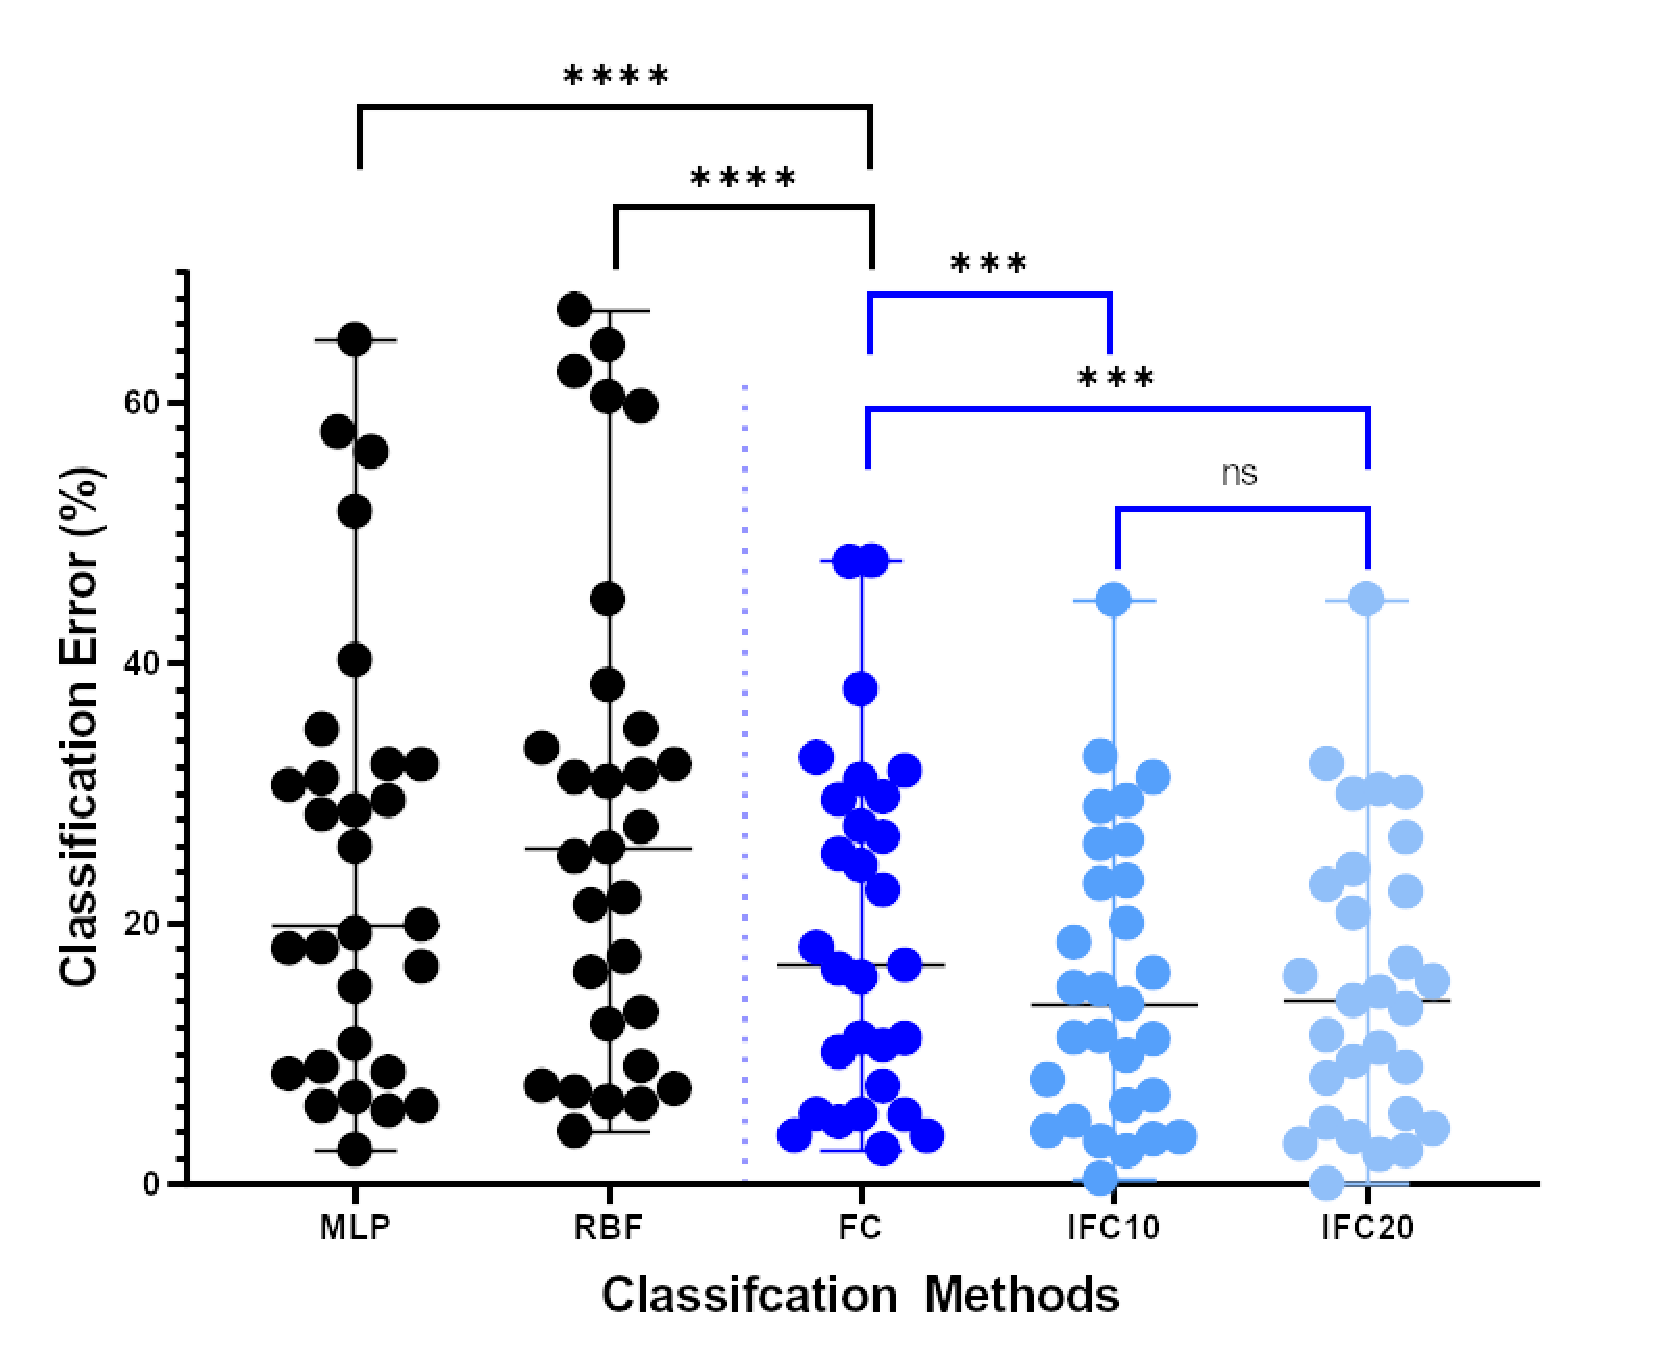
\includegraphics[scale=0.5]{ifc_scatter}
\par\end{centering}
\caption{Comparison of Classification Error Percentages for Different Machine
Learning Methods. The scatter plot displays individual classification
error measurements for each method (MLP, RBF, FC, IFC10, IFC20) with
lines indicating median values. Statistical significance is denoted
by asterisks, with '' indicating p \textless{} 0.0001, '{*}' indicating
p \textless{} 0.001, '' p \textless{} 0.01, and 'ns' indicating no
significant difference. The results show that FC significantly outperforms
both MLP and RBF, IFC10 improves upon FC, and there is no significant
difference between the IFC10 and IFC20 methods.\label{fig:ifc_scatter}}

\end{figure}

The scatter plot (Figure \ref{fig:ifc_scatter}) effectively demonstrates
the comparative performance of various classification methods in terms
of classification error percentage. The methods evaluated are Multi-Layer
Perceptron (MLP), Radial Basis Function (RBF), the simple feature
construction technique (FC), and two variants of the proposed modification
named IFC10 and IFC20 respectively. The FC method shows a lower median
classification error compared to both MLP and RBF, with the differences
being statistically significant (as indicated by the asterisks). This
suggests that the FC method outperforms MLP and RBF in terms of classification
accuracy. When comparing FC to IFC10, IFC10 displays a lower median
classification error, and the difference is statistically significant,
suggesting that IFC10 is an improvement over the standard FC method.
Between IFC10 and IFC20, the median classification errors are close,
and the lack of asterisks ('ns' for not significant) between these
two methods indicates that the difference in classification error
is not statistically significant. This suggests that the critical
parameter change from IFC10 to IFC20 does not have a significant impact
on classification accuracy.
\begin{figure}[H]
\begin{centering}
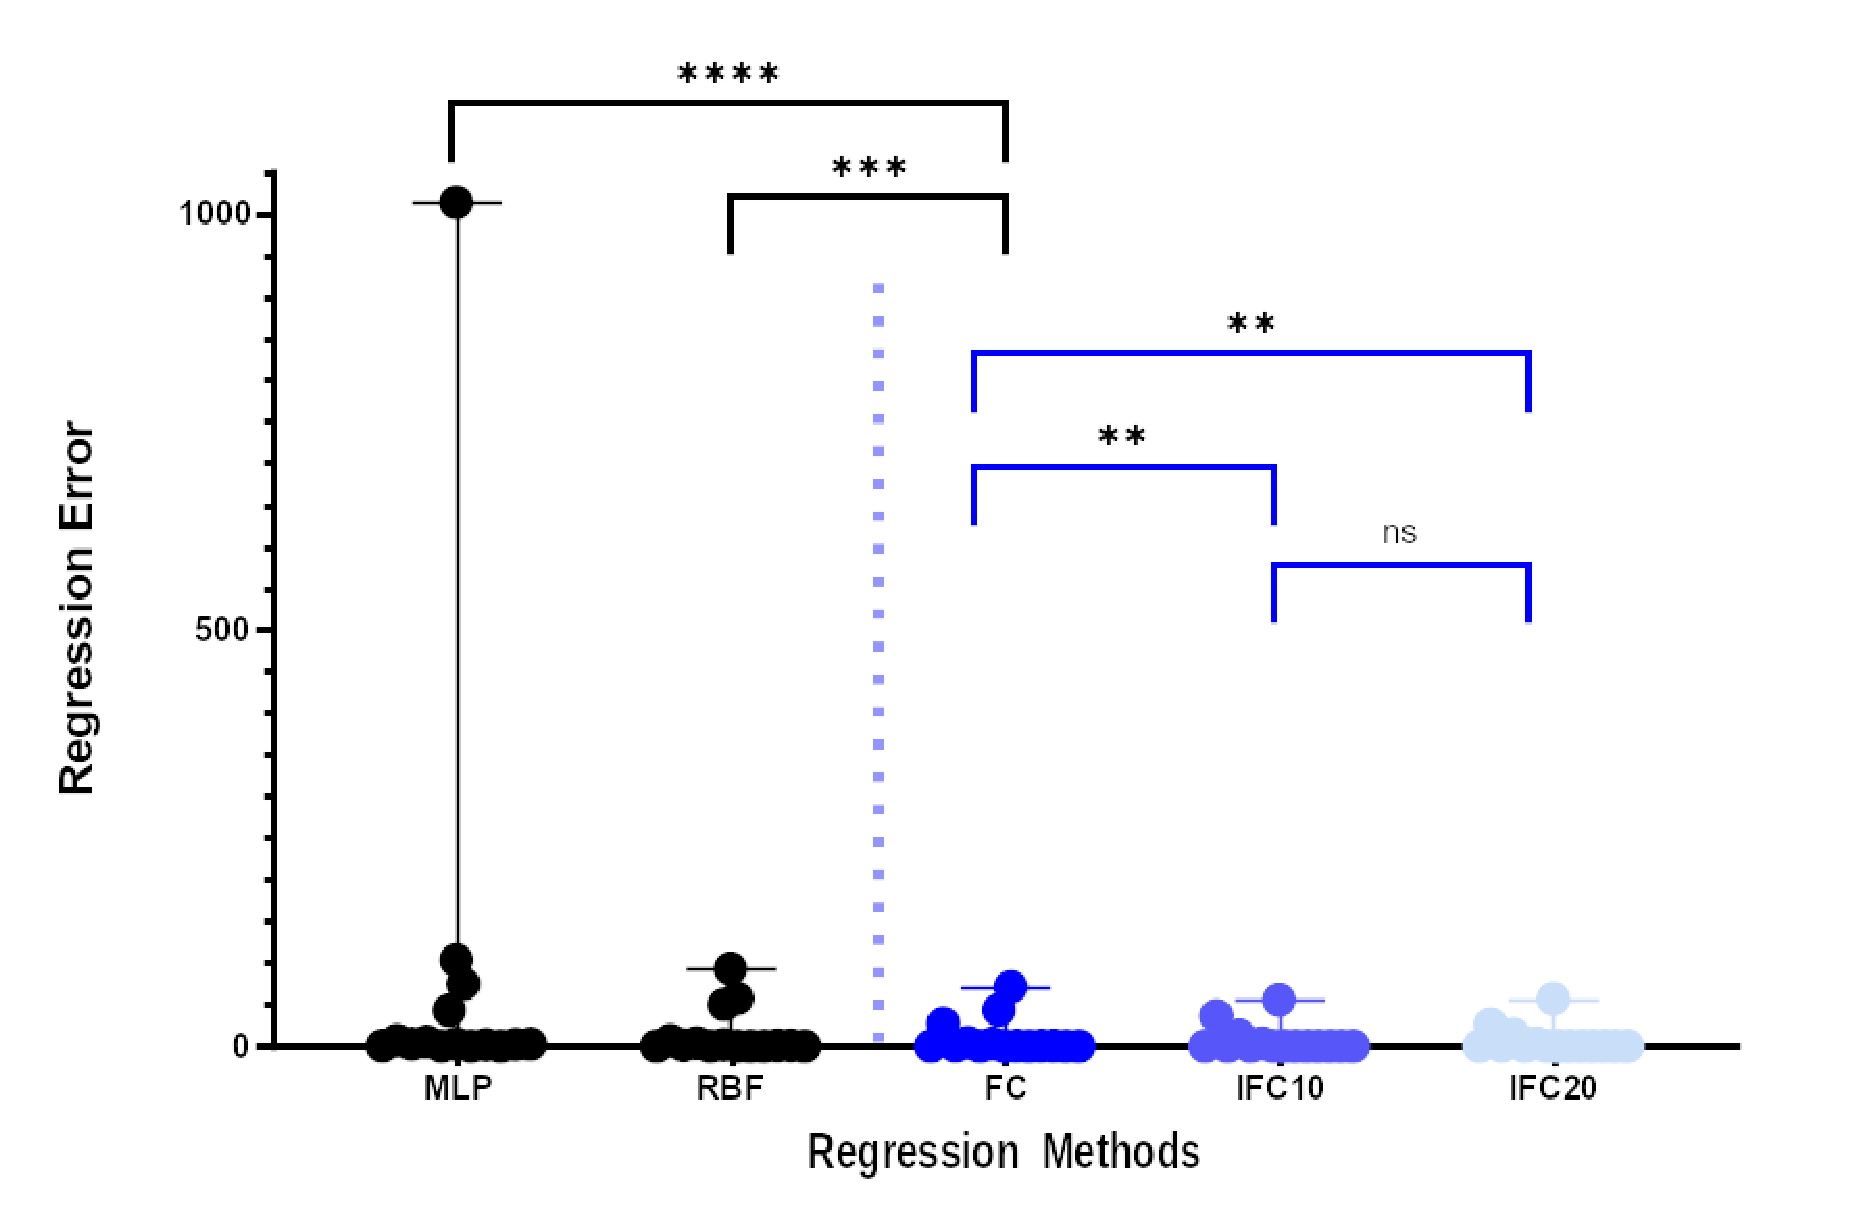
\includegraphics[scale=0.5]{ifc_regression}
\par\end{centering}
\caption{Comparative scatter plot of regression errors for machine learning
methods: Multi-Layer Perceptron (MLP), Radial Basis Function (RBF),
FC and Interval Feature Construction with parameters 10 (IFC10) and
20 (IFC20). The data points represent individual measurements of regression
error, with lines indicating the median values. Statistical significance
is denoted by asterisks, with FC showing significantly lower errors
than MLP and RBF, IFC10 improving upon FC, and no significant difference
between IFC10 and IFC20.\label{fig:scatter_regression}}

\end{figure}

The Figure \ref{fig:scatter_regression} depicts a scatter plot that
compares regression errors across the used machine learning regression
methods in the experiments. From the plot, we can see that:
\begin{itemize}
\item The FC method has a lower median regression error than both the MLP
and RBF methods. This is statistically significant, as indicated by
the asterisks ({*}{*} for p \textless{} 0.01 between FC and RBF, and
{*}{*}{*} for p \textless{} 0.001 between FC and MLP), suggesting
that FC is indeed a better method compared to MLP and RBF. 
\item The IFC10 method shows a lower median regression error compared to
the FC method, with this difference being statistically significant
({*}{*} for p \textless{} 0.01). This suggests that IFC10 is a better
method compared to FC. 
\item Between IFC10 and IFC20, the median regression error is similar, and
the difference is not statistically significant (ns for not significant).
This indicates that there is no significant difference in regression
error between IFC10 and IFC20 when the parameter is changed from 10
to 20.
\end{itemize}

\section{Conclusions\label{sec:Conclusions} }

In the current work, an efficient technique was proposed to identify
the bounding box of the values of chromosomes in Grammatical Evolution.
The proposed method precedes Grammatical Evolution and aims to discover
a promising value interval for the chromosome values and, in this
way, will significantly reduce the computational time required afterward
but at the same time make the research more efficient. The method
was tested on the Feature Construction technique, which is guided
by Grammatical Evolution. Experimental results and statistical comparison
show a significant reduction in classification error and data fitting
error using the proposed technique. In addition, from the statistical
comparison of the results, it appears that there is no direct effect
of the number of generations of the genetic algorithm on the effectiveness
of the method, which means that only a few generations are enough
to effectively find the promising value interval. Although the proposed
technique was applied to the feature generation method, it is quite
general and in the future it will be able to be applied to other application
areas of Grammatical Evolution such as the construction of artificial
neural networks, the rule generation method, etc. However, a major
drawback of the present technique is that it requires a significant
amount of computing resources for its execution, but this can be alleviated
by using parallel computing techniques, such as the MPI programming
library \citep{MPI} or the OpenMP library \citep{OpenMP}.

\vspace{6pt}


\authorcontributions{I.G.T., A.T. and E.K. conceived the idea and methodology and supervised
the technical part regarding the software. I.G.T. conducted the experiments,
employing several datasets, and provided the comparative experiments.
A.T. performed the statistical analysis. E.K. and all other authors
prepared the manuscript. E.K. and I.G.T. organized the research team
and A.T. supervised the project. All authors have read and agreed
to the published version of the manuscript.}

\funding{This research received no external funding.}

\institutionalreview{Not applicable.}

\informedconsent{Not applicable. }

\institutionalreview{Not applicable.}

\acknowledgments{This research has been financed by the European Union : Next Generation
EU through the Program Greece 2.0 National Recovery and Resilience
Plan , under the call RESEARCH -- CREATE -- INNOVATE, project name
“iCREW: Intelligent small craft simulator for advanced crew training
using Virtual Reality techniques\textquotedbl{} (project code:TAEDK-06195}

\appendixtitles{}

\appendixstart{}

\appendix

\begin{adjustwidth}{-\extralength}{0cm}{}

\reftitle{References}

\begin{thebibliography}{99}
\bibitem{Holland1}J.H. Holland, Genetic algorithms. Scientific american
\textbf{267}, pp. 66-73, 1992.

\bibitem{Stender}J. Stender, Parallel Genetic Algorithms:Theory \&
Applications. Edition: IOS Press, 1993. 

\bibitem{genetic1}D. Goldberg, Genetic Algorithms in Search, Optimization
and Machine Learning, Addison-Wesley Publishing Company, Reading,
Massachussets, 1989.

\bibitem{genetic2}Z. Michaelewicz, Genetic Algorithms + Data Structures
= Evolution Programs. Springer - Verlag, Berlin, 1996.

\bibitem{ge1}M. O’Neill, C. Ryan, Grammatical evolution, IEEE Trans.
Evol. Comput. \textbf{5,}pp. 349--358, 2001.

\bibitem{bnf1}J. W. Backus. The Syntax and Semantics of the Proposed
International Algebraic Language of the Zurich ACM-GAMM Conference.
Proceedings of the International Conference on Information Processing,
UNESCO, 1959, pp.125-132.

\bibitem{ge_program1}C. Ryan, J. Collins, M. O’Neill, Grammatical
evolution: Evolving programs for an arbitrary language. In: Banzhaf,
W., Poli, R., Schoenauer, M., Fogarty, T.C. (eds) Genetic Programming.
EuroGP 1998. Lecture Notes in Computer Science, vol 1391. Springer,
Berlin, Heidelberg, 1998.

\bibitem{ge_program2}M. O’Neill, M., C. Ryan, Evolving Multi-line
Compilable C Programs. In: Poli, R., Nordin, P., Langdon, W.B., Fogarty,
T.C. (eds) Genetic Programming. EuroGP 1999. Lecture Notes in Computer
Science, vol 1598. Springer, Berlin, Heidelberg, 1999.

\bibitem{ge_credit}A. Brabazon, M. O'Neill, Credit classification
using grammatical evolution, Informatica \textbf{30.3}, 2006.

\bibitem{ge_intrusion}S. Şen, J.A. Clark. A grammatical evolution
approach to intrusion detection on mobile ad hoc networks, In: Proceedings
of the second ACM conference on Wireless network security, 2009.

\bibitem{ge_water}L. Chen, C.H. Tan, S.J. Kao, T.S. Wang, Improvement
of remote monitoring on water quality in a subtropical reservoir by
incorporating grammatical evolution with parallel genetic algorithms
into satellite imagery, Water Research \textbf{ 42}, pp. 296-306,
2008.

\bibitem{ge_trig}C. Ryan, M. O’Neill, J.J. Collins, Grammatical evolution:
Solving trigonometric identities, proceedings of Mendel. Vol. 98.
1998.

\bibitem{ge_music}A.O. Puente, R. S. Alfonso, M. A. Moreno, Automatic
composition of music by means of grammatical evolution, In: APL '02:
Proceedings of the 2002 conference on APL: array processing languages:
lore, problems, and applications July 2002 Pages 148--155. 

\bibitem{ge_nn}Lídio Mauro Limade Campo, R. Célio Limã Oliveira,Mauro
Roisenberg, Optimization of neural networks through grammatical evolution
and a genetic algorithm, Expert Systems with Applications \textbf{56},
pp. 368-384, 2016.

\bibitem{ge_nn2}K. Soltanian, A. Ebnenasir, M. Afsharchi, Modular
Grammatical Evolution for the Generation of Artificial Neural Networks,
Evolutionary Computation \textbf{30}, pp 291--327, 2022.

\bibitem{ge_constant}I. Dempsey, M.O' Neill, A. Brabazon, Constant
creation in grammatical evolution, International Journal of Innovative
Computing and Applications \textbf{1} , pp 23--38, 2007.

\bibitem{ge_pacman}E. Galván-López, J.M. Swafford, M. O’Neill, A.
Brabazon, Evolving a Ms. PacMan Controller Using Grammatical Evolution.
In: , et al. Applications of Evolutionary Computation. EvoApplications
2010. Lecture Notes in Computer Science, vol 6024. Springer, Berlin,
Heidelberg, 2010.

\bibitem{ge_supermario}N. Shaker, M. Nicolau, G. N. Yannakakis, J.
Togelius, M. O'Neill, Evolving levels for Super Mario Bros using grammatical
evolution, 2012 IEEE Conference on Computational Intelligence and
Games (CIG), 2012, pp. 304-31.

\bibitem{ge_energy}D. Martínez-Rodríguez, J. M. Colmenar, J. I. Hidalgo,
R.J. Villanueva Micó, S. Salcedo-Sanz, Particle swarm grammatical
evolution for energy demand estimation, Energy Science and Engineering
\textbf{8}, pp. 1068-1079, 2020.

\bibitem{ge_comb}N. R. Sabar, M. Ayob, G. Kendall, R. Qu, Grammatical
Evolution Hyper-Heuristic for Combinatorial Optimization Problems,
IEEE Transactions on Evolutionary Computation \textbf{17}, pp. 840-861,
2013.

\bibitem{ge_crypt}C. Ryan, M. Kshirsagar, G. Vaidya, G. et al. Design
of a cryptographically secure pseudo random number generator with
grammatical evolution. Sci Rep \textbf{12}, 8602, 2022.

\bibitem{ge_decision}P.J. Pereira, P. Cortez, R. Mendes, Multi-objective
Grammatical Evolution of Decision Trees for Mobile Marketing user
conversion prediction, Expert Systems with Applications \textbf{168},
114287, 2021.

\bibitem{ge_analog}F. Castejón, E.J. Carmona, Automatic design of
analog electronic circuits using grammatical evolution, Applied Soft
Computing \textbf{62}, pp. 1003-1018, 2018.

\bibitem{ge_structured1}N. Lourenço, F.B. Pereira, E, Costa, Unveiling
the properties of structured grammatical evolution, Genetic Programming
and Evolvable Machines \textbf{17} , pp. 251-289, 2016.

\bibitem{ge_structured2}N. Lourenço, F. Assunção, F.B. Pereira, E.
Costa, P. Machado, Structured grammatical evolution: a dynamic approach,
Handbook of grammatical evolution, pp. 137-161, 2018.

\bibitem{pso1}Riccardo Poli, James Kennedy kennedy, Tim Blackwell,
Particle swarm optimization An Overview, Swarm Intelligence \textbf{1},
pp 33-57, 2007. 

\bibitem{ge_swarm1}M. O’Neill, A. Brabazon, Grammatical swarm: The
generation of programs by social programming. Natural Computing \textbf{5},
pp. 443-462, 2006.

\bibitem{ge_swarm2}E. Ferrante, E. Duéñez-Guzmán, A.E. Turgut, T.
Wenseleers, GESwarm: Grammatical evolution for the automatic synthesis
of collective behaviors in swarm robotics. In Proceedings of the 15th
annual conference on Genetic and evolutionary computation, pp. 17-24,
2013.

\bibitem{ge_par1}O. Popelka, P. Osmera, Parallel Grammatical Evolution
for Circuit Optimization. In: Hornby, G.S., Sekanina, L., Haddow,
P.C. (eds) Evolvable Systems: From Biology to Hardware. ICES 2008.
Lecture Notes in Computer Science, vol 5216. Springer, Berlin, Heidelberg.
https://doi.org/10.1007/978-3-540-85857-7\_40

\bibitem{ge_par2}P. Ošmera, Two level parallel grammatical evolution,
Advances in Computational Algorithms and Data Analysis pp. 509-525,
2009.

\bibitem{ge_geva}M. O'Neill, E. Hemberg, C. Gilligan, E. Bartley,
J. McDermott, A. Brabazon, GEVA: grammatical evolution in Java. ACM
SIGEVOlution \textbf{3}, pp. 17-22, 2008.

\bibitem{ge_gramevol}F. Noorian, A.M. de Silva, P.H.W. Leong, gramEvol:
Grammatical Evolution in R, Journal of Statistical Software \textbf{71},
pp. 1--26, 2016.

\bibitem{ge_gelab}M.A. Raja, C. Ryan, GELAB - A Matlab Toolbox for
Grammatical Evolution. In: Yin, H., Camacho, D., Novais, P., Tallón-Ballesteros,
A. (eds) Intelligent Data Engineering and Automated Learning -- IDEAL
2018. IDEAL 2018. Lecture Notes in Computer Science(), vol 11315,
2018. Springer, Cham. https://doi.org/10.1007/978-3-030-03496-2\_22

\bibitem{ge_genclass}N.Anastasopoulos, I.G. Tsoulos, A. Tzallas,
GenClass: A parallel tool for data classification based on Grammatical
Evolution, SoftwareX \textbf{16}, 100830, 2021.

\bibitem{ge_qfc}I.G. Tsoulos, QFC: A Parallel Software Tool for Feature
Construction, Based on Grammatical Evolution, Algorithms \textbf{15},
295, 2022.

\bibitem{tsoulos_dnc}N. Anastasopoulos, I.G. Tsoulos, E. Karvounis,
A. Tzallas, Locate the Bounding Box of Neural Networks with Intervals,
Neural Process Lett \textbf{52}, pp. 2241--2251, 2020. 

\bibitem{fc1}Dimitris Gavrilis, Ioannis G. Tsoulos, Evangelos Dermatas,
Selecting and constructing features using grammatical evolution, Pattern
Recognition Letters \textbf{29},pp. 1358-1365, 2008. 

\bibitem{fc2}Dimitris Gavrilis, Ioannis G. Tsoulos, Evangelos Dermatas,
Neural Recognition and Genetic Features Selection for Robust Detection
of E-Mail Spam, Advances in Artificial Intelligence Volume 3955 of
the series Lecture Notes in Computer Science pp 498-501, 2006.

\bibitem{fc3}George Georgoulas, Dimitris Gavrilis, Ioannis G. Tsoulos,
Chrysostomos Stylios, João Bernardes, Peter P. Groumpos, Novel approach
for fetal heart rate classification introducing grammatical evolution,
Biomedical Signal Processing and Control \textbf{2},pp. 69-79, 2007 

\bibitem{fc4}Otis Smart, Ioannis G. Tsoulos, Dimitris Gavrilis, George
Georgoulas, Grammatical evolution for features of epileptic oscillations
in clinical intracranial electroencephalograms, Expert Systems with
Applications \textbf{38}, pp. 9991-9999, 2011 

\bibitem{fc5}A. T. Tzallas, I. Tsoulos, M. G. Tsipouras, N. Giannakeas,
I. Androulidakis and E. Zaitseva, Classification of EEG signals using
feature creation produced by grammatical evolution, In: 24th Telecommunications
Forum (TELFOR), pp. 1-4, 2016.

\bibitem{nn1}C. Bishop, Neural Networks for Pattern Recognition,
Oxford University Press, 1995.

\bibitem{nn2}G. Cybenko, Approximation by superpositions of a sigmoidal
function, Mathematics of Control Signals and Systems \textbf{2}, pp.
303-314, 1989.

\bibitem{rbf1}J. Park and I. W. Sandberg, Universal Approximation
Using Radial-Basis-Function Networks, Neural Computation 3, pp. 246-257,
1991.

\bibitem{rbf2}H. Yu, T. Xie, S. Paszczynski, B. M. Wilamowski, Advantages
of Radial Basis Function Networks for Dynamic System Design, in IEEE
Transactions on Industrial Electronics \textbf{58}, pp. 5438-5450,
2011.

\bibitem{doublecrossover}Z. Michaelewicz, Genetic Algorithms + Data
Structures = Evolution Programs. Springer - Verlag, Berlin, 1996.

\bibitem{UCL}M. Kelly, R. Longjohn, K. Nottingham, The UCI Machine
Learning Repository. 2023. Available online: https://archive.ics.uci.edu
(accessed on 18 February 2024).

\bibitem{Keel}J. Alcalá-Fdez, A. Fernandez, J. Luengo, J. Derrac,
S. García, L. Sánchez, F. Herrera. KEEL Data-Mining Software Tool:
Data Set Repository, Integration of Algorithms and Experimental Analysis
Framework. Journal of Multiple-Valued Logic and Soft Computing 17,
pp. 255-287, 2011.

\bibitem{appendicitis}Weiss, Sholom M. and Kulikowski, Casimir A.,
Computer Systems That Learn: Classification and Prediction Methods
from Statistics, Neural Nets, Machine Learning, and Expert Systems,
Morgan Kaufmann Publishers Inc, 1991.

\bibitem{australian}J.R. Quinlan, Simplifying Decision Trees. International
Journal of Man-Machine Studies \textbf{27}, pp. 221-234, 1987. 

\bibitem{balance}T. Shultz, D. Mareschal, W. Schmidt, Modeling Cognitive
Development on Balance Scale Phenomena, Machine Learning \textbf{16},
pp. 59-88, 1994.

\bibitem{cleveland1}Z.H. Zhou,Y. Jiang, NeC4.5: neural ensemble based
C4.5,\textquotedbl{} in IEEE Transactions on Knowledge and Data Engineering
\textbf{16}, pp. 770-773, 2004.

\bibitem{cleveland2}R. Setiono , W.K. Leow, FERNN: An Algorithm for
Fast Extraction of Rules from Neural Networks, Applied Intelligence
\textbf{12}, pp. 15-25, 2000.

\bibitem{dermatology}G. Demiroz, H.A. Govenir, N. Ilter, Learning
Differential Diagnosis of Eryhemato-Squamous Diseases using Voting
Feature Intervals, Artificial Intelligence in Medicine. \textbf{13},
pp. 147--165, 1998.

\bibitem{heart}I. Kononenko, E. Šimec, M. Robnik-Šikonja, Overcoming
the Myopia of Inductive Learning Algorithms with RELIEFF, Applied
Intelligence \textbf{7}, pp. 39--55, 1997

\bibitem{hayesroth}B. Hayes-Roth, B., F. Hayes-Roth. Concept learning
and the recognition and classification of exemplars. Journal of Verbal
Learning and Verbal Behavior \textbf{16}, pp. 321-338, 1977.

\bibitem{housevotes}R.M. French, N. Chater, Using noise to compute
error surfaces in connectionist networks: a novel means of reducing
catastrophic forgetting, Neural Comput. \textbf{14}, pp. 1755-1769,
2002.

\bibitem{ion1}J.G. Dy , C.E. Brodley, Feature Selection for Unsupervised
Learning, The Journal of Machine Learning Research \textbf{5}, pp
845--889, 2004.

\bibitem{ion2}S. J. Perantonis, V. Virvilis, Input Feature Extraction
for Multilayered Perceptrons Using Supervised Principal Component
Analysis, Neural Processing Letters \textbf{10}, pp 243--252, 1999.

\bibitem{liver} J. Garcke, M. Griebel, Classification with sparse
grids using simplicial basis functions, Intell. Data Anal. \textbf{6},
pp. 483-502, 2002.

\bibitem{mammographic}M. Elter, R. Schulz-Wendtland, T. Wittenberg,
The prediction of breast cancer biopsy outcomes using two CAD approaches
that both emphasize an intelligible decision process, Med Phys. \textbf{34},
pp. 4164-72, 2007.

\bibitem{parkinsons}M.A. Little, P.E. McSharry, E.J. Hunter, J. Spielman,
L.O. Ramig, Suitability of dysphonia measurements for telemonitoring
of Parkinson's disease. IEEE Trans Biomed Eng. \textbf{56}, pp. 1015-1022,
2009.

\bibitem{pima}J.W. Smith, J.E. Everhart, W.C. Dickson, W.C. Knowler,
R.S. Johannes, Using the ADAP learning algorithm to forecast the onset
of diabetes mellitus, In: Proceedings of the Symposium on Computer
Applications and Medical Care IEEE Computer Society Press, pp.261-265,
1988.

\bibitem{popfailures}D.D. Lucas, R. Klein, J. Tannahill, D. Ivanova,
S. Brandon, D. Domyancic, Y. Zhang, Failure analysis of parameter-induced
simulation crashes in climate models, Geoscientific Model Development
\textbf{6}, pp. 1157-1171, 2013.

\bibitem{regions}N. Giannakeas, M.G. Tsipouras, A.T. Tzallas, K.
Kyriakidi, Z.E. Tsianou, P. Manousou, A. Hall, E.C. Karvounis, V.
Tsianos, E. Tsianos, A clustering based method for collagen proportional
area extraction in liver biopsy images (2015) Proceedings of the Annual
International Conference of the IEEE Engineering in Medicine and Biology
Society, EMBS, 2015-November, art. no. 7319047, pp. 3097-3100. 

\bibitem{saheart}T. Hastie, R. Tibshirani, Non-parametric logistic
and proportional odds regression, JRSS-C (Applied Statistics) \textbf{36},
pp. 260--276, 1987.

\bibitem{segment}M. Dash, H. Liu, P. Scheuermann, K. L. Tan, Fast
hierarchical clustering and its validation, Data \& Knowledge Engineering
\textbf{44}, pp 109--138, 2003.

\bibitem{student}P. Cortez, A. M. Gonçalves Silva, Using data mining
to predict secondary school student performance, In Proceedings of
5th FUture BUsiness TEChnology Conference (FUBUTEC 2008) (pp. 5--12).
EUROSIS-ETI, 2008.

\bibitem{transfusion}I-Cheng Yeh, King-Jang Yang, Tao-Ming Ting,
Knowledge discovery on RFM model using Bernoulli sequence, Expert
Systems with Applications \textbf{36}, pp. 5866-5871, 2009.

\bibitem{wdbc}W.H. Wolberg, O.L. Mangasarian, Multisurface method
of pattern separation for medical diagnosis applied to breast cytology,
Proc Natl Acad Sci U S A. \textbf{87}, pp. 9193--9196, 1990.

\bibitem{wine1}M. Raymer, T.E. Doom, L.A. Kuhn, W.F. Punch, Knowledge
discovery in medical and biological datasets using a hybrid Bayes
classifier/evolutionary algorithm. IEEE transactions on systems, man,
and cybernetics. Part B, Cybernetics : a publication of the IEEE Systems,
Man, and Cybernetics Society, \textbf{33} , pp. 802-813, 2003.

\bibitem{wine2}P. Zhong, M. Fukushima, Regularized nonsmooth Newton
method for multi-class support vector machines, Optimization Methods
and Software \textbf{22}, pp. 225-236, 2007.

\bibitem{eeg}R.G. Andrzejak, K. Lehnertz, F. Mormann, C. Rieke, P.
David, and C. E. Elger, Indications of nonlinear deterministic and
finite-dimensional structures in time series of brain electrical activity:
Dependence on recording region and brain state, Phys. Rev. E \textbf{64},
pp. 1-8, 2001.

\bibitem{zoo}M. Koivisto, K. Sood, Exact Bayesian Structure Discovery
in Bayesian Networks, The Journal of Machine Learning Research\textbf{
5}, pp. 549--573, 2004.

\bibitem{abalone}W. J Nash, T.L. Sellers, S.R. Talbot, A.J. Cawthor,
W.B. Ford, The Population Biology of Abalone (\_Haliotis\_ species)
in Tasmania. I. Blacklip Abalone (\_H. rubra\_) from the North Coast
and Islands of Bass Strait, Sea Fisheries Division, Technical Report
No. 48 (ISSN 1034-3288), 1994.

\bibitem{airfoil}T.F. Brooks, D.S. Pope, A.M. Marcolini, Airfoil
self-noise and prediction. Technical report, NASA RP-1218, July 1989. 

\bibitem{concrete}I.Cheng Yeh, Modeling of strength of high performance
concrete using artificial neural networks, Cement and Concrete Research.
\textbf{28}, pp. 1797-1808, 1998. 

\bibitem{key23}D. Harrison and D.L. Rubinfeld, Hedonic prices and
the demand for clean ai, J. Environ. Economics \& Management \textbf{5},
pp. 81-102, 1978.

\bibitem{powell}M.J.D Powell, A Tolerant Algorithm for Linearly Constrained
Optimization Calculations, Mathematical Programming \textbf{45}, pp.
547-566, 1989. 

\bibitem{MPI}W. Gropp, E. Lusk, N. Doss, A. Skjellum, A high-performance,
portable implementation of the MPI message passing interface standard,
Parallel Computing 22, pp. 789-828, 1996.

\bibitem{OpenMP}L. Dagum, R. Menon, OpenMP: an industry standard
API for shared-memory programming, IEEE Computational Science and
Engineering 5, pp. 46-55, 1998.

\end{thebibliography}

\end{adjustwidth}{}
\end{document}
